
   \section{Object Deletion}

   \begin{frame}
      \frametitle{Object Deletion}
      \begin{center}
      \Huge{Object Deletion}
      \end{center}
   \end{frame}
   
   \begin{frame}
      \frametitle{Object Deletion}
      \begin{itemize}
         \item TrickHLA supports notification of HLA object deletions.
         \item An HLA object can be deleted as a result of a federate resigning
         or by explicit deletion by the federate.
         \item Using TrickHLA object deletion consists of three steps:
         \begin{itemize}
            \item Step 1: Extend the \texttt{TrickHLA::ObjectDeleted} class
            and implement the \texttt{deleted()} virtual function.
            \item Step 2: In the \texttt{S\_define} file add an object-deleted
            object to each simulation object that needs to be notified of a
            deletion.
            \item Step 3: Configure object deleted in the \texttt{input.py} file.
         \end{itemize}
      \end{itemize}
   \end{frame}

   \begin{frame}[fragile]
      \frametitle{Ownership Transfer}
      \framesubtitle{Step 1: Extend the \texttt{TrickHLA::ObjectDeleted} Class}
      \begin{itemize}
         \item Step 1: Extend the \texttt{TrickHLA::ObjectDeleted} class and
         implement the \texttt{deleted()} virtual function.
         \item Example in \texttt{SineObjectDeleted.hh}:
      \end{itemize}
\begin{Verbatim}[frame=single, fontsize=\scriptsize]
#include "TrickHLA/include/TrickHLAObjectDeleted.hh”

class SineObjectDeleted : public TrickHLAObjectDeleted
{
...
  public:
...
   void deleted(                // RETURN: -- None.
        TrickHLAObject * obj ); // IN:     -- Deleted object.
};
\end{Verbatim}
   \end{frame}

   \begin{frame}[fragile]
      \frametitle{Ownership Transfer}
      \framesubtitle{Step 1: Extend the \texttt{TrickHLA::ObjectDeleted} Class (Continued)}
      \begin{itemize}
         \item Step 1 continued: Example in \texttt{SineObjectDeleted.cpp}:
      \end{itemize}
\begin{Verbatim}[frame=single, fontsize=\scriptsize]
void SineObjectDeleted::deleted( // RETURN: -- None.
   TrickHLAObject * obj)         // IN: -- Object which was deleted.
{
   std::ostringstream msg;
   msg << "SineObjectDeleted::deleted() Object '" << obj->get_name()
       << "' deleted from the federation.";
   send_hs( stdout, (char *) msg.str().c_str() );
}
\end{Verbatim}
   \end{frame}

   \begin{frame}[fragile]
      \frametitle{Ownership Transfer}
      \framesubtitle{Step 2: Add Object-deleted Object to \texttt{S\_define}}
      \begin{itemize}
         \item Step 2: In the \texttt{S\_define} file add an object-deleted
         object to each simulation object that needs to be notified of a deletion.
      \end{itemize}
\begin{Verbatim}[frame=single, fontsize=\scriptsize]
   class ASimObject : public Trick::SimObject {
      ...
      SineData     sim_data;
      SineData     lag_comp_data;
      SineOwnershipHandler   ownership_handler;
      SinePacking            packing;
      SineLagCompensation    lag_compensation;
      SineInteractionHandler interaction_handler;
      SineObjectDeleted      obj_deleted_callback;

      ASimObject() {
        P50 ("initialization") packing.initialize( &sim_data );
        P50 ("initialization") lag_compensation.initialize( &sim_data, 
                                                            &lag_comp_data );
        ...
      }
   };
\end{Verbatim}
   \end{frame}

   \begin{frame}[fragile]
      \frametitle{Ownership Transfer}
      \framesubtitle{Step 3: Configuration}
      \begin{itemize}
         \item Step 3: Configure object deleted in the \texttt{input} file.
         \item In the \texttt{RUN\_a\_side/input.py} file:
\begin{Verbatim}[frame=single, fontsize=\scriptsize]
THLA.manager.objects[0].deleted = A.obj_deleted_callback
THLA.manager.objects[1].deleted = P.obj_deleted_callback
\end{Verbatim}
         \item In the \texttt{RUN\_p\_side/input.py} file:
\begin{Verbatim}[frame=single, fontsize=\scriptsize]
THLA.manager.objects[0].deleted = A.obj_deleted_callback
THLA.manager.objects[1].deleted = P.obj_deleted_callback
\end{Verbatim}
      \end{itemize}
   \end{frame}
   
   \begin{frame}
      \frametitle{Object Deletion}
      \framesubtitle{TrickHLA jobs in THLA.sm}
      \begin{figure}
      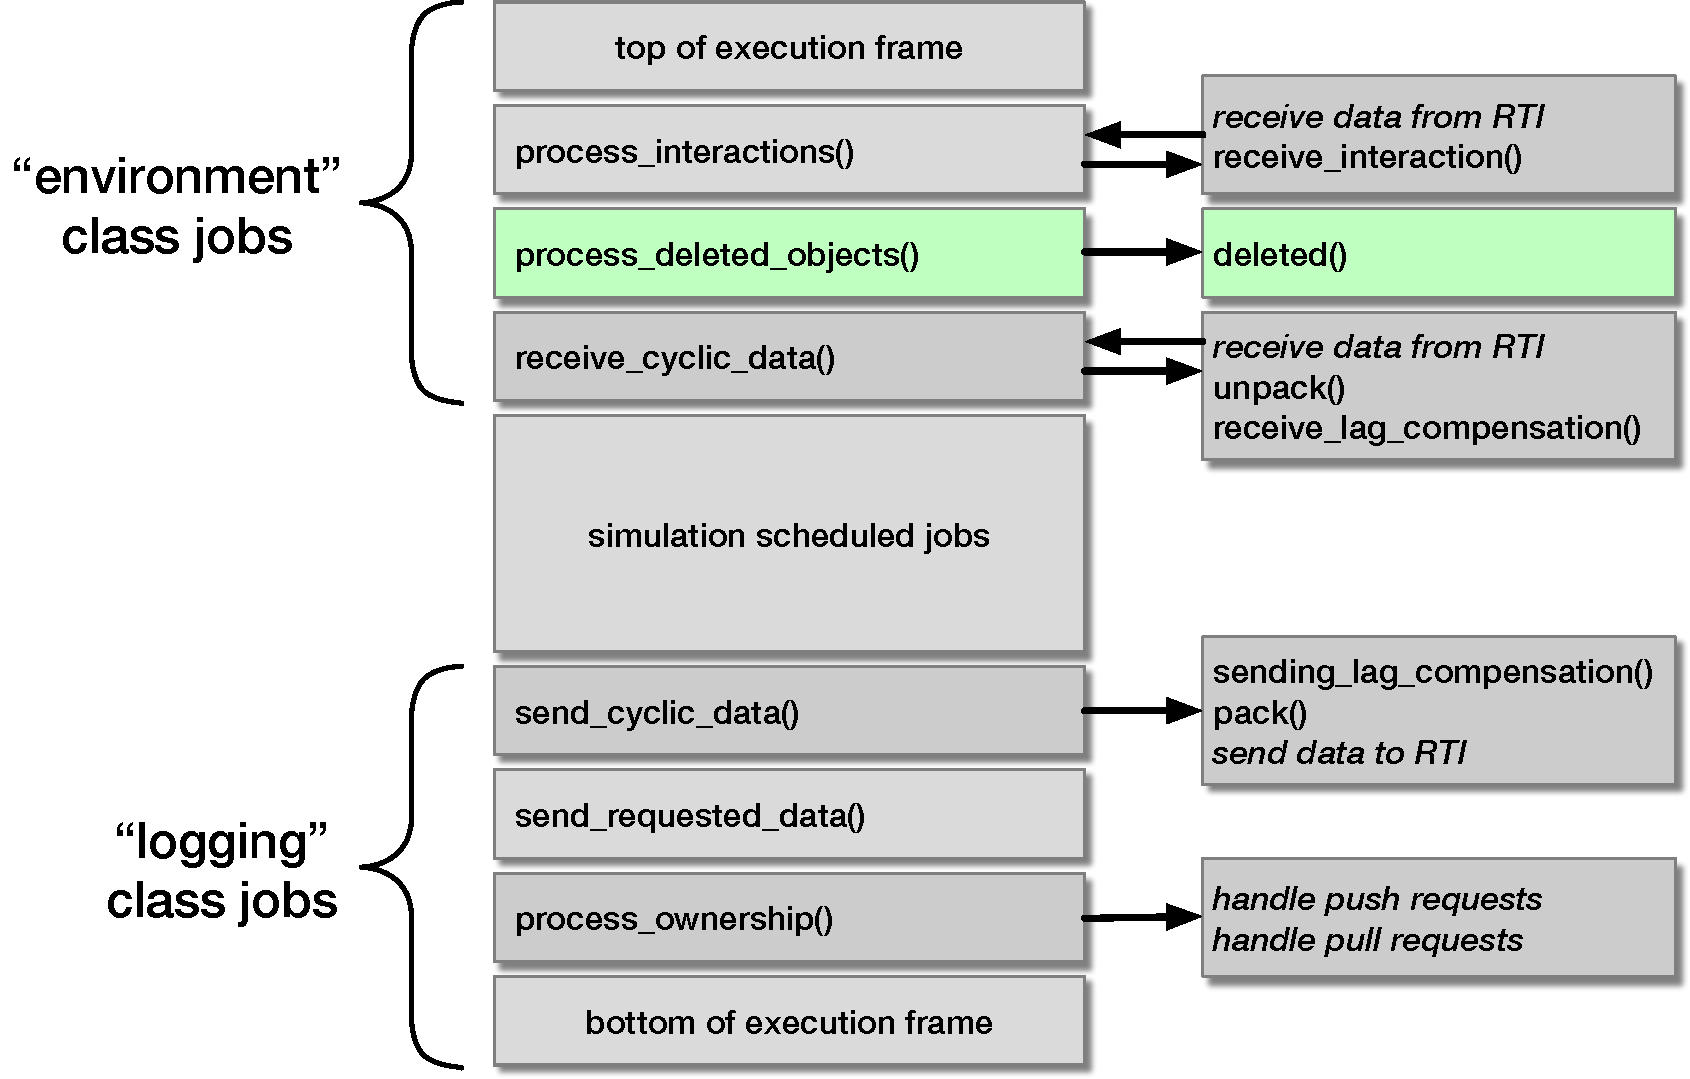
\includegraphics[scale=0.4]{TutorialTHLADeletedJobs.pdf}
      \end{figure}
   \end{frame}
